\documentclass{article}
\usepackage{tabularx}
\usepackage{pdflscape}
\usepackage{graphicx}

\graphicspath{ {./} }

\newcolumntype{s}{>{\hsize=0.2\hsize}>{\centering}X}
\newcolumntype{m}{>{\hsize=1.0\hsize}>{\centering}X}
\newcolumntype{b}{>{\hsize=1.8\hsize}>{\centering}X}

% Enter the name of the subject
\newcommand{\assignmentname}{Assignment 4: Testing}
% Your names
\newcommand{\studentA}{Evelien Daems}
\newcommand{\studentB}{Lars Van Roy}

\title{\textmd{\textbf{Software Engineering}}\\\normalsize\vspace{0.1in}\Large{\assignmentname}\\\vspace{0.1in}\small{\textit{3 Ba INF \  2018-2019}}}
\author{\studentA \\ \studentB}

\begin{document}
\maketitle
\noindent
\underline{Control Flow Graph}\newline
\newline
Een control flow graph is een visuele weergave van een programma waarmee alle mogelijke paden doorheen een programma kunnen gegenereerd worden. Elke binaire node (een node waar twee pijlen uitkomen) komt overheen met een conditie in het programma. Elke mogelijke sequentie van nodes dat eindigt in een eindstaat is een mogelijk pad door het programma, het is echter niet gegarandeerd dat dit pad ook bestaat. Sommige condities kunnen enkel slagen indien andere condities ook slagen en of slagen sowieso x aantal keren. Het is dus niet omdat de sequentie bestaat in de control flow graph dat het ook een mogelijk pad is. Voor de flow graph van de calculate() functie zie appendix A. \\
\newline
\maketitle
\noindent
\underline{Cyclomatic Complexity}\newline
\newline
De cyclomatic complexity kan berekend worden door het aantal edges - het aantal nodes te beschouwen + 2 of het aantal binaire conditie nodes + 1. Beide geven ons in dit geval 10. Deze waarde symboliseert een bovengrens voor het aantal mogelijke onafhankelijke paden door de flowgraph. \\
aantal edges - aantal nodes + 2 = 29 - 21 + 2 = 10 \\
aantal binarie condities + 1 = 9 + 1 = 10 \\

\newpage
\maketitle
\noindent
\underline{independent paths}\newline
\newline
Wanneer we beginnend van het kortst mogelijke pad verdergaan door steeds een nieuw onafhankelijke pad te nemen krijgen we een mogelijkheid om de verschillende paden voor te stellen. Een nieuw pad wordt onafhankelijk genoemd van de voorgaande paden als er in het nieuwe pad een node voorkomt die nog niet voorkwam in de voorgaande paden. Wanneer we dit doen bekomen we de volgende paden. \\

\begin{table}[h]
	\centering
	\begin{tabularx}{\linewidth}{| s | b |}
		\hline
		index & pad \tabularnewline
		\hline
		0 & {1, 2, 6, 7, 21} \tabularnewline
		\hline
		1 & {1, 2, 6, 7, 8, 9, 10, 7, 21} \tabularnewline
		\hline
		2 & {1, 2, 3, 2, 6, 7, 8, 9, 10, 7, 21} \tabularnewline
		\hline
		3 & {1, 2, 3, 4, 5, 2, 6, 7, 21} \tabularnewline
		\hline
		4 & {1, 2, 3, 4, 5, 2, 6, 7, 8, 9, 10, 11, 12, 10, 7, 21} \tabularnewline
		\hline
		5 & {1, 2, 3, 4, 5, 2, 6, 7, 8, 9, 10, 11, 12, 13, 14, 12, 10, 7, 21} \tabularnewline
		\hline
		6 & {1, 2, 3, 4, 5, 2, 6, 7, 8, 9, 10, 11, 12, 13, 14, 15, 12, 10, 7, 21} \tabularnewline
		\hline
		7 & {1, 2, 3, 4, 5, 2, 6, 7, 8, 9, 10, 11, 12, 13, 14, 15, 16, 17, 12, 10, 7, 21} \tabularnewline
		\hline
		8 & {1, 2, 3, 4, 5, 2, 6, 7, 8, 9, 10, 11, 12, 13, 14, 15, 16, 17, 18, 12, 10, 7, 21} \tabularnewline
		\hline
		9 & {1, 2, 3, 4, 5, 2, 6, 7, 8, 9, 10, 11, 12, 13, 14, 15, 16, 17, 18, 19, 20, 12, 10, 12, 10, 7, 10, 12, 10, 7, 21} \tabularnewline
		\hline
	\end{tabularx}
	\caption{alle mogelijke paden}
\end{table}

\newpage
\maketitle
\noindent
\underline{test cases}\newline
\newline
Bij nadere observatie van deze paden zien we dat het merendeel hiervan niet bereikbaar is. sommige condities kunnen niet falen zonder dat andere in het programma ook falen en omgekeerd. Uiteindelijk blijven volgende 4 paden over met bijhorende input en output. Hierbij zijn triviale inputvelden, of m.a.w. inputvelden waarvoor de waarde niet relevant is om het gewenste pad te bekomen, weggelaten.\\

\begin{table}[h]
	\centering
	\begin{tabularx}{\linewidth}{| s | b | m |}
		\hline
		index & input & output \tabularnewline
		\hline
		1 & m\_db\.m\_tidlist = \{\} & \{\{\}, \{\}\} \tabularnewline
		\hline
		2 & m\_db\.m\_tidlist = \{0:\{0\}\}; \newline min\_sup = 2; & \{\{\}, \{\}\} \tabularnewline
		\hline
		4 & m\_db\.m\_tidlist = \{0:\{0\}\}; \newline min\_sup = 1; & \{\{[0]\}, \{\}\} \tabularnewline
		\hline
		9 & m\_db\.m\_tidlist = \{0:\{1,2\}, 1:\{1\}\}; \newline min\_sup = 1; & \{\{[0], [1]\}, \{[0, 1]\}, \{\}\} \tabularnewline
		\hline
	\end{tabularx}
	\caption{test cases}
\end{table}

\newpage
\maketitle
\noindent
\underline{appendix A}\newline
\newline
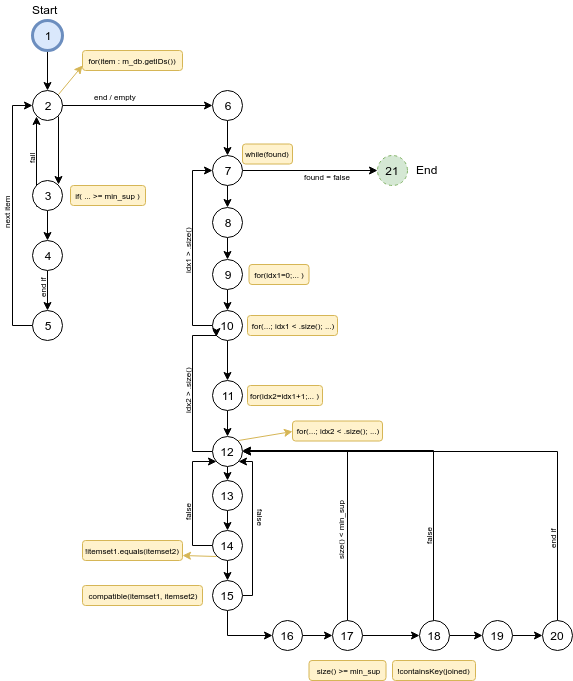
\includegraphics[width=\textwidth]{control_flow_graph}

\newpage
\begin{landscape}
	\maketitle
	\noindent
	\underline{appendix B}\newline
	\newline
	\begin{table}[h]
		\centering
		\begin{tabularx}{\linewidth}{| >{\hsize=0.3\hsize}>{\centering}X | >{\hsize=1.35\hsize}>{\centering}X | >{\hsize=1.35\hsize}>{\centering}X | >{\hsize=1\hsize}>{\centering}X |}
			\hline
			index & pad & input & output \tabularnewline
			\hline
			0 & {1, 2, 6, 7, 21} & bestaat niet & bestaat niet\tabularnewline
			\hline
			1 & {1, 2, 6, 7, 8, 9, 10, 7, 21} & m\_db\.m\_tidlist = \{\} & \{\{\}, \{\}\} \tabularnewline
			\hline
			2 & {1, 2, 3, 2, 6, 7, 8, 9, 10, 7, 21} & m\_db\.m\_tidlist = \{0:\{0\}\}; \newline min\_sup = 2; & \{\{[0]\}, \{\}\} \tabularnewline
			\hline
			3 & {1, 2, 3, 4, 5, 2, 6, 7, 21} & bestaat niet & bestaat niet \tabularnewline
			\hline
			4 & {1, 2, 3, 4, 5, 2, 6, 7, 8, 9, 10, 11, 12, 10, 7, 21} & m\_db\.m\_tidlist = \{0:\{0\}\}; \newline min\_sup = 1; & \{\{[0]\}, \{\}\} \tabularnewline
			\hline
			5 & {1, 2, 3, 4, 5, 2, 6, 7, 8, 9, 10, 11, 12, 13, 14, 12, 10, 7, 21} & bestaat niet & bestaat niet\tabularnewline
			\hline
			6 & {1, 2, 3, 4, 5, 2, 6, 7, 8, 9, 10, 11, 12, 13, 14, 15, 12, 10, 7, 21} & bestaat niet & bestaat niet \tabularnewline
			\hline
			7 & {1, 2, 3, 4, 5, 2, 6, 7, 8, 9, 10, 11, 12, 13, 14, 15, 16, 17, 12, 10, 7, 21} & bestaat niet & bestaat niet \tabularnewline
			\hline
			8 & {1, 2, 3, 4, 5, 2, 6, 7, 8, 9, 10, 11, 12, 13, 14, 15, 16, 17, 18, 12, 10, 7, 21} & bestaat niet & bestaat niet \tabularnewline
			\hline
			9 & {1, 2, 3, 4, 5, 2, 6, 7, 8, 9, 10, 11, 12, 13, 14, 15, 16, 17, 18, 19, 20, 12, 10, 12, 10, 7, 10, 12, 10, 7, 21} & bestaat niet & bestaat niet \tabularnewline
			\hline
		\end{tabularx}
		\caption{paden + test cases}
	\end{table}
\end{landscape}

\end{document}